%% Journal of Open Research Software Latex template -- Created By Stephen Bonner and John Brennan, Durham University, UK.

\documentclass{jors}
\usepackage{amsmath, amssymb}
\usepackage{cite}
\usepackage{graphicx, subcaption}
\graphicspath{ {images/} }

%% Set the header information
\pagestyle{fancy}
\definecolor{mygray}{gray}{0.6}
\renewcommand\headrule{}
\rhead{\footnotesize 3}
\rhead{\textcolor{gray}{UP JORS software Latex paper template version 0.1}}

\begin{document}

{\bf Software paper for submission to the Journal of Open Research Software} \\

Please submit the completed paper to: editor.jors@ubiquitypress.com

\rule{\textwidth}{1pt}

\section{(1) Overview}

\vspace{0.5cm}

\section{Title}
spinsim: a GPU optimised simulator of spin half and spin one quantum systems

\section{Paper Authors}
1. Tritt, Alex;\\
2. Morris, Joshua;\\
3. Hochstetter, Joel;\\
4. Anderson, R. P.;\\
5. Saunderson, James;\\
6. Turner, L. D.;\\

\section{Paper Author Roles and Affiliations}
1. School of Physics \& Astronomy, Monash University, Victoria 3800, Australia.\\
	Primary author of the released packages.\\
2. School of Physics \& Astronomy, Monash University, Victoria 3800, Australia.\\
	Present address: Faculty of Physics, University of Vienna, 1010 Vienna, Austria.\\
	Author of first version of code.\\
3. School of Physics \& Astronomy, Monash University, Victoria 3800, Australia.\\
	Present address: School of Physics, University of Sydney, NSW 2006, Australia.\\
	Optimization and extension to spin one of first version of code.\\
4. School of Molecular Sciences, La Trobe University, PO box 199, Bendigo, Victoria 3552, Australia.\\
	Original conception of first version of code.\\
5. Department of Electrical and Computer Systems Engineering, Monash University, Victoria 3800, Australia.\\
	Advice on numerical analysis.\\
6. School of Physics \& Astronomy, Monash University, Victoria 3800, Australia.\\
	Original conception of released version of algorithm.

\section{Abstract}
	\texttt{spinsim} is a \emph{python} package that simulates spin half and spin one quantum mechanical systems following a time dependent Shroedinger equation. It makes use of \texttt{numba.cuda} \cite{lam_numba_2015}, which is an \emph{LLVM} (Low Level Virtual Machine) \cite{lattner_llvm_2004} compiler, and other optimisations, to allow for fast and accurate evaluation on \emph{Nvidia Cuda} \cite{nickolls_scalable_2008} compatible systems using GPU parallelisation. \texttt{spinsim} is available for installation on \emph{PyPI}, and the source code is available on \emph{github}. The initial use case for the package will be to simulate quantum sensing-based Bose Einstein condensate (BEC) experiments for the Monash University School of Physics and Astronomy spinor BEC lab, but we anticipate it will be useful in simulating any range of spin half or spin one quantum systems with time dependent Hamiltonians that cannot be solved analytically. These appear in the fields of nuclear magnetic resonance (NMR), nuclear quadrupole resonance (NQR) and magnetic resonance imaging (MRI) experiments and quantum sensing, and with the spin one systems of nitrogen vacancy centres (NVCs) and BECs.

\section{Keywords}
Time dependent Schroedinger equation; Spin one; Spin half; Integrator; GPU; Solver; python; numba;

\section{Introduction}
\subsection{Motivation}
	Ultracold rubidium atoms have proven their effectiveness in state of the art technologies in quantum sensing \cite{degen_quantum_2017}, the use of quantum mechanics to make precise measurements of small signals. The rotation of these atoms can be modelled as quantum spin systems, which is the quantum mechanical model for objects with angular momentum. The simplest spin system, spin half (ie spin quantum number of \(\frac12\), also referred to as a qubit), is quantised into just two quantum spin levels, and this describes the motion of some fundamental particles such as electrons. However, systems more practical for sensing, such as ultracold rubidium atoms, are more accurately described as a spin one quantum system (ie spin quantum number of \(1\), also referred to as a quitrit), which is quantised into three quantum spin levels.
	
	The design of sensing protocols requires many steps of verification, including simulation. This is especially important, since running real experiments can be expensive and time consuming, and thus it is more practical to debug such protocols quickly and cheaply on a computer. In general, any design of experiments using spin systems could benefit from a fast, accurate method of simulation.

	% \texttt{AtomicPy} \cite{morris_qcmonkatomicpy_2018}
	In the past, the spinor Bose Einstein condensate (spinor BEC) lab at Monash University used an in-house, \emph{cython} based script, on which this package is based, and standard differential equation solvers (such as \emph{Mathematica}'s function \texttt{NDSolve}) to solve the Schroedinger equation for quantum sensing spin systems. Spin one systems are sometimes approximated to spin half for a faster execution time, at the cost of modelling all effects of the system. However, these methods are not completely optimised for our use case, and therefore come with some issues.

	First, while the execution time for these solvers is acceptable for running a small number of experiments, for certain experiments involving large arrays of independent atom clouds (which require many thousands of simulations to be run), this time accumulates to the order of many hours, or even multiple days.

	Second, the Schroedinger equation has the geometric property of being norm persevering. In other words, the time evolution operator for a system between two points in time must be unitary. As such, numerical solutions to the Schroedinger equation should also preserve this property. For many numerical methods like those in the Runge Kutta family, the approximations used might not be norm preserving, and the evaluated quantum state may diverge towards an infinite norm, or converge to zero if run for many iterations.

	Third, our system (and similar spin systems) can be very oscillatory. In standard conditions for our application, the expected spin projection of a system that we want to solve for can rotate in physical space (alternatively viewed as a point rotating around an abstract object known as a \emph{Bloch sphere}) at a rate of 700kHz. Standard integration methods require very small time steps in order to accurately depict these oscillations.

\section{Implementation and architecture}
	% \subsection{Mathematical methods}
	\subsection{Quantum mechanics background}
		\texttt{spinsim} solves the time-dependent Schr\"{o}dinger equation

		\begin{align}
			i\hbar\frac{\mathrm{d}\psi(t)}{\mathrm{d}t} &= H(t)\psi(t),\label{eq:schroedinger}
		\end{align}

		where the quantum state \(\psi(t) \in \mathbb{C}^N\) is assumed normalised, and the Hamiltonian \(H(t) \in \mathbb{C}^{N \times N}\) is Hermitian. Here \(N\) is the number of levels in the quantum system. Often we are considering systems with spin \(S\). Here spin-half is the \(N = 2\) case, and spin-one is \(N = 3\). We set \(\hbar = 1\), so that the Hamiltonian has units 
		
		% Furthermore, we have chosen for the Hamiltonian \(H(t)\) to have the physical dimension of frequency, rather than the more typical dimension of energy. To elaborate, we represent energies \(E\) of the system as their equivalent frequencies \(f\) from the Planck relation
		
		\begin{align}
			E &= \hbar \omega\\
			&= 2\pi\hbar f,
		\end{align}
		
		% where \(\hbar\) is (reduced) Planck's constant (or equivalently, setting 
		% \(\hbar = 1\)). In addition, rather than being represented by standard coordinates in \(\mathbb{C}^{N \times N}\), in \texttt{spinsim} the Hamiltonian \(H(t)\) is instead represented with respect to a choice of basis for the corresponding Lie Algebra, \(\mathfrak{su}(N)\). For example, when set to spin half mode, the \texttt{spinsim} package solves the time dependent Schroedinger equation of the form
		Rather than ... parametrizing the problem ... we consider time varying real coefficients in a linear combination of fixed operators,

		\begin{align}
			H(t) &= \sum_{j = 1}^{N^2 - 1} a_j(t) A_j.
		\end{align}
		
		It is well known that ... spin in magnetic field has ... . We exclude the identity ... energy zero point.

		In the spin one case there is no standard basis ... . Choices include Gell Mann, quadrupole basis, ... . In general ... Lie algebra ... mathfrak ... admits a basis ... .
		% \begin{align}
		% 	\frac{\mathrm{d}}{\mathrm{d}t}\psi(t) = -i 2\pi (f_x(t) J_x + f_y(t) J_y + f_z(t) J_z) \psi(t),
		% \end{align}

		where \(i^2 = -1\), \(\psi(t) \in \mathbb{C}^2\), and the spin half spin projection operators are given by


		DONT WRITE OUT, sigma
		\begin{align}
			J_x &= \frac12\begin{pmatrix}
				0 & 1 \\
				1 & 0
			\end{pmatrix},
			&J_y &= \frac12\begin{pmatrix}
				0 & -i \\
				i &  0
			\end{pmatrix},
			&\textrm{and }J_z &= \frac12\begin{pmatrix}
				1 &  0 \\
				0 & -1
			\end{pmatrix}.\label{eq:spin_half_operators}
		\end{align}

		Call omega, no implementation detail
		% The fields \(f\) that represents the time dependent Hamiltonian \(H(t)\), are the collection of energy functions \(f_x(t), f_y(t), f_z(t)\), with time \(t\) and \(f\) with physical dimension of frequency that control the dynamics of the system. The user must define a method that returns a sample of these field functions when a sampling time is input. In physical terms, these functions could represent the \(x,y,z\) components of a magnetic field applied to a magnetically spin one BEC or NVC.

		Similarly, when \texttt{spinsim} is set to spin one mode, it can solve the Schroedinger equation of the form

		\begin{align}
			\frac{\mathrm{d}}{\mathrm{d}t}\psi(t) = -i 2\pi (f_x(t) J_x + f_y(t) J_y + f_z(t) J_z + f_q(t) Q) \psi(t).
		\end{align}

		where now \(\psi(t) \in \mathbb{C}^3\), and the spin one operators are given by

		\begin{align}
			J_x &= \frac{1}{\sqrt{2}}\begin{pmatrix}
				0 & 1 & 0 \\
				1 & 0 & 1 \\
				0 & 1 & 0
			\end{pmatrix},&
			J_y &= \frac{1}{\sqrt{2}}\begin{pmatrix}
				0 & -i &  0 \\
				i &  0 & -i \\
				0 &  i &  0
			\end{pmatrix},\nonumber\\
			J_z &= \begin{pmatrix}
				1 & 0 &  0 \\
				0 & 0 &  0 \\
				0 & 0 & -1
			\end{pmatrix},&
			\textrm{and }Q &= \frac{1}{3}\begin{pmatrix}
				1 &  0 & 0 \\
				0 & -2 & 0 \\
				0 &  0 & 1
			\end{pmatrix}.\label{eq:spin_one_operators}
		\end{align}

		The matrices \(J_x, J_y, J_z\) are regular spin operators, and \(Q\) is a quadrupole operator. Note that \(Q\) is proportional to \(Q_{zz}\) as defined by Hamley et al \cite{hamley_spin-nematic_2012}, and \(Q_0\) as defined by Di et al \cite{di_dipolequadrupole_2010}.
		INLINE Q DIAG. WHY WE'VE PICKED THESE FOUR. For ground state spin one atoms in a magnetic field, ... Breit Rabi ... . COULD BE READILY EXTENDED TO INCLUDE FURTHER ELEMENTS OR TO HIGHER SPINS.
		
		% Too far out of scope
		% Alternative: integrate Bloch equations 3 coupled real equations
		% fast and parallel function from wavefunctions
		Frequently when one calculates the times series of the quantum state \(\psi(t)\), they are also interested in its expected spin projection \(\left\langle J\right\rangle\)(t). It is given by the vector

		% Inline
		\begin{align}
			\left\langle J\right\rangle(t) &= \begin{pmatrix}
				\psi(t)^\dagger J_x \psi(t)\\
				\psi(t)^\dagger J_y \psi(t)\\
				\psi(t)^\dagger J_z \psi(t)
			\end{pmatrix},
		\end{align}

		where \(\cdot^\dagger\) is the adjoint operator (also referred to as Hermitian conjugate, and is implemented as complex conjugate transpose). The expected spin projection can be interpreted as the average direction that the spin system is oriented in space when many systems of the equivalent state are measured (due to the Heisenberg uncertainty principle, only one component of the exact orientation of a quantum state can be known at any point in time, which is why we need to deal with expected values rather than absolute values). However, it can also be used to model the overall orientation of an ensemble of many quantum systems, like a BEC, for instance. \texttt{spinsim} has the functionality to calculate the expected spin projection of a system from its state.
	
	\subsection{Unitary time evolution and the Magnus expansion}
		Given that \(\psi(t)\) is a unit vector, it is possible to write \(\psi(t)\) in terms of a unitary transformation \(U(t, t_0)\) of the state \(\psi(t_0)\), for any time \(t_0\). In other words, for any \(t_0,t \in \mathbb{R}\), there is a unitary transformation \(U(t, t_0)\) such that
		
		\begin{align}
			\psi(t) &= U(t, t_0)\psi(t_0).
		\end{align}

		From Equation \eqref{eq:schroedinger}, \(U(t, t_0)\) also follows the Schroedinger equation via

		\begin{align}
			\frac{\mathrm{d}}{\mathrm{d}t}U(t, t_0)\psi(t_0) &= -i2\pi H(t)U(t, t_0)\psi(t_0)\textrm{ for any }\psi(t_0)\in\mathbb{C}^N,\textrm{ so}\\
			\frac{\mathrm{d}}{\mathrm{d}t}U(t, t_0) &= -i2\pi H(t)U(t, t_0).\label{eq:unitary_schroedinger}
		\end{align}

		Thus, to solve Equation \eqref{eq:schroedinger} for \(\psi(t)\) given a particular \(\psi(t_0)\), one only needs to solve Equation \eqref{eq:unitary_schroedinger} for \(U(t, t_0)\). Note that because \(U(t, t_0)\) is unitary, the calculated value of \(\psi(t)\) using this method will not change in magnitude, conserving probability.

		Also since \(U(t, t_0)\) is unitary (and continuous in time \(t\)), it can be written as a matrix exponential of a skew Hermitian matrix. For example, if the Hamiltonian \(H(t)\) is constant in time (and a real linear combination of Hermitian matrices defined by Equations \eqref{eq:spin_half_operators} or \eqref{eq:spin_one_operators}), then the solution would be

		\begin{align}
			U(t, t_0) &= \exp(-i2\pi H(t - t_0)).
		\end{align}

		The act of integrating a linear differential equation by exponentiation can be generalised for time dependent Hamiltonians using the Magnus Series \cite{blanes_magnus_2009}, where
		
		\begin{align}
			U(t, t_0) &= \exp(-i2\pi G(t - t_0))\\
			&= \exp(-i2\pi \sum_{m = 1}^\infty G_m(t - t_0)),
		\end{align}

		where \(G(t)\) is a series of \(G_m(t)\), each of which are a function of \(H\) and its commutators. \(G_1(t)\), for example, is just \(G_1(t) = H_\mathrm{av}t\), where \(H_\mathrm{av}\) is the average value of \(H\) over the interval being integrated over, which is the solution for when \(H\) is constant in time. The terms \(G_m(t)\) for \(m > 1\) are corrections to this approximation. One can truncate the Magnus series before infinity to make a Mangus expansion, which can given an approximation for \(U(t, t_0)\). Importantly, any truncation of the Magnus expansion is unitary, meaning that probability will be conserved when used.

		Something else to note about unitary time evolution operators, is that they can be broken into a product of multiple other time evolution operators via

		\begin{align}
			U(t, t_0) &= U(t, t_1)U(t_1, t_0).
		\end{align}

		Each of these parts can be approximated as a Magnus expansion. So, if the Magnus expansion of time evolution operator is inaccurate, it can be broken down into a product of many time evolution operators which each make a much smaller step between times. These components will each have a much more accurate Magnus expansion.

		In fact, many unitary time stepping techniques have been developed based on the Magnus expansion \cite{auer_magnus_2018}. Some of these techniques use Gauss-Legendre quadrature sampling to avoid the integration of commutators of the Hamiltonian, producing simple expressions that can be used for unitary time stepping. In particular, we used the commutator free 4 (CF4) from \cite{auer_magnus_2018} as our integration method. Suppose we wish to evaluate a short time step of \(U(t_f + \mathrm{d}t, t_f)\) by taking a short step \(\mathrm{d}t\) from a fine sample time \(t_f\). Then as part of the CF4 method, the field functions are sampled at particular times based on the second order Gauss-Legendre quadrature, given by
			
		\begin{align}
			t_1 &= t_f + \frac12 \mathrm{d}t\left(1 - \frac{1}{\sqrt{3}}\right)\textrm{, and}\\
			t_2 &= t_f + \frac12 \mathrm{d}t\left(1 + \frac{1}{\sqrt{3}}\right).
		\end{align}
		
		Then given the matrices
		
		\begin{align}
			\overline{G}_1 &= 2\pi\mathrm{d}t\left(\frac{3 + 2\sqrt{3}}{12}H(t_1) + \frac{3 - 2\sqrt{3}}{12}H(t_2)\right)\textrm{, and}\label{eq:cf4_sample_1}\\
			\overline{G}_2 &= 2\pi\mathrm{d}t\left(\frac{3 - 2\sqrt{3}}{12}H(t_1) + \frac{3 + 2\sqrt{3}}{12}H(t_2)\right),\label{eq:cf4_sample_2}
		\end{align}

		the unitary time step can be calculated using

		\begin{align}
			U(t_f + \mathrm{d}t, t_f) = \exp(-i\overline{G}_2)\exp(-i\overline{G}_1).\label{eq:cf4_implementation}
		\end{align}

	\subsection{Exponentiator}
		From Equation \eqref{eq:cf4_implementation}, evaluating matrix exponentials is a core part of the integration algorithm. However, the \texttt{spinsim} package uses the user provided field functions \(f(t)\) as a vector representation of the Hamiltonian of the spin system being simulated, rather than generic matrix elements in an array. This allows for implementation of matrix exponentiation that takes advantage of this representation. For all implementations of exponentiation, the \texttt{spinsim} computes the matrix exponential
		
		\begin{align}
			E(g) &= E(g_x, g_y, g_z, g_q)\\
			&= \exp(-i (g_x J_x + g_y J_y + g_z J_z + g_q Q)).
		\end{align}
		
		In practice, \(g\) is the Lie algebra (spin and quadrature) basis representation of \(\overline{G_1}\) or \(\overline{G_2}\) defined in Equations \eqref{eq:cf4_sample_1} and \eqref{eq:cf4_sample_2}, which need to be exponentiated in Equation \eqref{eq:cf4_implementation}. For spin half, the default exponentiator is in an analytic form. For spin one, an exponentiator based on the Lie Trotter product formula \cite{moler_nineteen_2003} is used instead. Explicitly, this formula is
		
		\begin{align}
			\exp\left( A + B\right) &= \lim_{n\to\infty} \left(\exp\left(\frac{A}{n}\right) \exp\left(\frac{B}{n}\right)\right)^n
		\end{align}
		
		Where \(A,B\in\mathbb{C}^{N\times N}\) are matrix operators, and \(n\in\mathbb{N}\). The equality holds for without the limit for all \(n\) if the operators commute, like it does for real and complex numbers. This tells us that we can approximate a matrix exponential of a linear combination of spin operators by reducing the size of the coefficients of these operators, taking the analytically simple exponentials of each of the operators \(-iJ_x, -iJ_y, -iJ_z\) and \(-iQ\) separately, multiplying each individual result together, and then raising the combination \(T\) to the power of the original reduction.
		
		For our spin one case, the exponential \(E(g)\) can be approximated as, for large \(2^\tau\),

		\begin{align}
			E(g) =& \exp\left(-ig_x J_x - ig_y J_y - ig_z J_z - ig_q Q\right)\\
			=& \exp\left(2^{-\tau}\left(-ig_x J_x - ig_y J_y - ig_z J_z - ig_q Q\right)\right)^{2^\tau}\\
			\approx& \biggl(\exp\left(-i\frac12\left(2^{-\tau} g_z J_z + 2^{-\tau}g_q Q\right)\right)\nonumber\\
			&\cdot\exp\left(-i\left(2^{-\tau} g_\phi J_\phi\right)\right)\nonumber\\
			&\cdot\exp\left(-i\frac12\left(2^{-\tau} g_z J_z + 2^{-\tau} g_q Q\right)\right)\biggr)^{2^\tau}\\
			=& \begin{pmatrix}
				\left(\frac{\Gamma}{PZ}\right)^2 & \frac{SP}{Z\Phi} & -\left(\frac{\Sigma P}{\Phi}\right)^2 \\
				\frac{SP\Phi}{Z} & CP^4 & \frac{SPZ}{\Phi} \\
				-\left(\frac{\Sigma \Phi}{P}\right)^2 & \frac{SPZ\Phi}{1} & \left(\frac{\Gamma Z}{P}\right)^2
			\end{pmatrix}^{2^\tau}\\
			=& T^{2^\tau}.
		\end{align}

		where

		\begin{align}
			g_\phi &= \sqrt{g_x^2 + g_y^2}&&\nonumber\\
			J_\phi &= \frac{g_x}{g_\phi}J_x + \frac{g_y}{g_\phi}J_y&&\nonumber\\
			\Gamma &= \cos\left(2^{-\tau} \frac{g_\phi}{2}\right) & \Phi &= \exp\left(i2^{-\tau}g_\phi\right)\nonumber\\
			\Sigma &= \sin\left(2^{-\tau} \frac{g_\phi}{2}\right) & Z &= \exp\left(i2^{-\tau}\frac{g_z}{2}\right)\nonumber\\
			C &= \cos\left(2^{-\tau} g_\phi\right) & P &= \exp\left(i2^{-\tau}\frac{g_q}{6}\right)\nonumber\\
			S &= \frac{-i}{\sqrt2}\sin\left(2^{-\tau} g_\phi\right)&&
		\end{align}
	
		Once \(T\) is calculated, it is then recursively squared \(\tau\) times to obtain \(E(g)\). The approach used for spin one exponentiation means that the package cannot solve arbitrary spin one quantum systems, as that would require the ability to exponentiate a point in the full, 8 dimensional Lie algebra of \(\mathfrak{su}(3)\), rather than just the four dimensional subspace spanned by the subalgebra \(\mathfrak{su}(2)\) spanned by \(\{J_x, J_y, J_z\}\), and the single quadratic operator \(Q\). Including the full algebra could be possible as a feature update if there is demand for it, though just including this subspace is sufficient for our application, and many others, and has the advantage of being able to use this faster, more specialised method of matrix exponentiation.

		Note that, the methods for both spin half and spin one use analytic forms of exponentials to construct the result, meaning that all calculated time evolution operators are unitary. This guarantees that the results of \texttt{spinsim} maintain unitary and conserve probability as required.

	\subsection{Discretisation and parallelisation}
		Consider quantising time with
		\begin{align}
			t_k &= t_0 + \mathrm{D}t\cdot k,
		\end{align}

		where \(\mathrm{D}t\) is the time step of the time series (in contrast to \(\mathrm{d}t\), a smaller time step for integration). If we define

		\begin{align}
			\psi_k = \psi(t_k)\textrm{ and}\\
			U_k = U(t_{k}, t_{k-1}),
		\end{align}
		
		then the time series of states \(\psi_k\) and time evolution operators \(U_k\) satisfies

		\begin{align}
			\psi_k &= U_k\psi_{k-1}\label{eq:integration_compilation}
		\end{align}

		This presents an opportunity for parallelism. While each of the \(\psi_k\) must be evaluated sequentially, the value of the \(U_k\) is independent of the value of any \(\psi_{k_0}\), or any other \(U_{k_0}\). This means that the time evolution operators \(U_k\) can all be calculated in parallel, and it allows \texttt{spinsim} to use GPU parallelisation on the level of time sample points, so a speed up is achieved even if just a single simulation is run.

		In summary, \texttt{spinsim} splits the time evolution of the full simulation into time evolution \(U_k\) within small time intervals \([t_{k - 1}, t_{k}]\), which are each calculated massively in parallel on a GPU. When all the \(U_k\) are calculated, the CPU then multiplies the \(U_k\) together (a comparatively less demanding job than calculating them) using Equation \eqref{eq:integration_compilation} to determine the \(\psi_k\).

		Beyond discretisation for parallelisation, we discretise our time evolution operator into individual integration time steps. So, each of the \(U_k\) are split into products of time evolution operators between times separated by the integration time step via
		
		\begin{align}
			U(t_k, t_{k-1}) &= U(t_k, t_k - \mathrm{d}t) \cdots U(t_{k-1} + 2\mathrm{d}t, t_{k-1} + \mathrm{d}t) U(t_{k-1} + \mathrm{d}t, t_{k-1})\\
			U_k &= u^k_{L-1} \cdots u^k_0\textrm{, where}\\
			u^k_{L-1} &= U(t_0 + (k - 1)\mathrm{D}t + (l + 1)\mathrm{d}t, t_0 + (k - 1)\mathrm{D}t + l\mathrm{d}t)
		\end{align}

		with \(\mathrm{d}t\) being the integration level time step. Note that the time steps are related to each other by \(\mathrm{D}t = L\mathrm{d}t\), where \(L\in\mathbb{N}\).

	\subsection{Rotating frame}
		If the rotating frame option is selected, the \(U_k\) are first calculated within a rotating frame of reference as \(U^r_k\), which, in some situations, reduces the size of the field functions used in the calculation, increasing accuracy. The rotation speed of the rotating frame is calculated locally for each parallel time step \(U_k\), and only for rotations around the \(z\) axis. The rotating from field functions \(f^r_x, f^r_y, f^r_z,\) and \(f^r_q\) are related to the field function from the user input via
		
		\begin{align}
			f^r_x(t) + if^r_y(t) &= e^{-i 2\pi f_r t}(f_x(t) + if_y(t)),\\
			f^r_z(t) &= f_z(t) - f_r\textrm{, and}\\
			f^r_q(t) &= f_q(t), \textrm{ for spin one.}
		\end{align}
		
		Where \(f_r = f_z(t_k + \frac12\mathrm{D}t)\) is sampled the midpoint value of the fields over the interval \([t_{k - 1}, t_k]\). This, assuming that a midpoint sample is representative of an average value over the time interval, decreases the magnitude of \(f_z(t)\), while leaving the other field components at an equivalent magnitude. The rotation is then applied to obtain the lab frame time evolution operator \(U_k\) via
		
		\begin{align}
			U_k &= \exp(-i 2 \pi f_r J_z \mathrm{D}t) U^r_k.
		\end{align}

		Specifically, this relationship is

		\begin{align}
			U_k &= \begin{pmatrix}
				e^{-i 2\pi f_r \mathrm{D}t} & 0 & 0\\
				0 & 1 & 0\\
				0 & 0 & e^{i 2\pi f_r \mathrm{D}t}
			\end{pmatrix} U^r_k, \textrm{ for spin one, and}\\
			U_k &= \begin{pmatrix}
				e^{-i \pi f_r \mathrm{D}t} & 0\\
				0 & e^{i \pi f_r \mathrm{D}t}
			\end{pmatrix} U^r_k, \textrm{ for spin half.}
		\end{align}

		It is a common technique in solving quantum mechanical problems to enter rotating frames, and their more abstract counterparts of interaction pictures \cite{j_j_sakurai_jun_john_modern_1994}. Note that this is typically done in conjunction with the Rotating Wave Approximation (RWA), which is an assumption that the oscillatory components of \(f^r_x, f^r_y, f^r_z,\) and \(f^r_q\) on an average of many cycles do not have a large contribution to time evolution of the solution and can be ignored. In some cases, this allows for analytic solutions to the approximate quantum system to be obtained. Note that the RWA is \emph{not} invoked in \texttt{spinsim}, as doing this would reduce the accuracy of simulation results, defeating our purpose of using a rotating frame.
		
	% \subsubsection{Magnus based integration method}
	% 	The integration method used in \texttt{spinsim} is the commutator free 4 (CF4) method from Auer et al \cite{auer_magnus_2018}, which based on the Magnus expansion. Each of the \(U_k\) are split into products of time evolution operators between times separated by a smaller time step, that is,
		
	% 	\begin{align}
	% 		U(t_k, t_{k-1}) &= U(t_k, t_k - \mathrm{d}t) \cdots U(t_{k-1} + 2\mathrm{d}t, t_{k-1} + \mathrm{d}t) U(t_{k-1} + \mathrm{d}t, t_{k-1})\\
	% 		U_k &= u^k_{L-1} \cdots u^k_0\textrm{, where}\\
	% 		u^k_{L-1} &= U(t_0 + (k - 1)\mathrm{D}t + (l + 1)\mathrm{d}t, t_0 + (k - 1)\mathrm{D}t + l\mathrm{d}t)
	% 	\end{align}

	% 	with \(\mathrm{d}t\) being the integration level time step. Note that the time steps are related to each other by \(\mathrm{D}t = L\mathrm{d}t\), where \(L\in\mathbb{N}\).

		% The CF4 method is used to calculate each individual \(u^k_l\). Let the fine sample time be given by \(t_f = l\mathrm{d}t + t_k\). Then as part of the CF4 method, the field functions are sampled at particular times based on the second order Gauss-Legendre quadrature, given by
		
		% \begin{align}
		% 	t_1 &= t_f + \frac12 \mathrm{d}t\left(1 - \frac{1}{\sqrt{3}}\right)\textrm{, and}\\
		% 	t_2 &= t_f + \frac12 \mathrm{d}t\left(1 + \frac{1}{\sqrt{3}}\right).
		% \end{align}

		% Now, let
		% \begin{align}
		% 	f(t_1) &= (f_x(t_1), f_y(t_1), f_z(t_1), f_q(t_1))\textrm{, and}
		% 	f(t_2) &= (f_x(t_2), f_y(t_2), f_z(t_2), f_q(t_2)).
		% \end{align}
		
		% The integration time evolution operator can then be calculated using
		
		% \begin{align}
		% 	g_1 =& (g_{1,x}, g_{1,y}, g_{1,z}, g_{1,q})\\
		% 	=& 2 \pi \mathrm{d}t \left(\frac{3 + 2 \sqrt{3}}{12} f(t_1) + \frac{3 - 2 \sqrt{3}}{12} f(t_2)\right)\textrm{, and}\\
		% 	g_2 =& (g_{2,x}, g_{2,y}, g_{2,z}, g_{2,q})\\
		% 	=& 2 \pi \mathrm{d}t \left(\frac{3 - 2 \sqrt{3}}{12} f(t_1) + \frac{3 + 2 \sqrt{3}}{12} f(t_2)\right)\textrm{, so}\\
		% 	u =& \exp(-i \left( g_{2,x} J_x + g_{2,y} J_y + g_{2,z} J_z + g_{2,q} Q\right))\\
		% 	&\cdot\exp(-i \left( g_{1,x} J_x + g_{1,y} J_y + g_{1,z} J_z + g_{1,q} Q\right)).
		% \end{align}

% \subsection{Software architecture}
	\subsection{Integrator architecture}
		The integrator in the \texttt{spinsim} package calls a \texttt{numba.cuda.jit()}ed kernel to be run on a \emph{Cuda} capable \emph{Nvidia} GPU in parallel, with a different thread being allocated to each of the \(U_k\). This returns when each of the \(U_k\) have been evaluated.
		
		The thread starts by calculating \(t_k\) and, if the rotating frame is being used, \(f_r\). The latter is done by sampling a (\texttt{numba.cuda.jit()}ed version of a) user provided \emph{python} function \(f\) describing how to sample the Hamiltonian. The code then loops over each integration time step \(\mathrm{d}t\) to calculate the integration time evolution operators \(u^k_l\).
		
		Within the loop, the integrator enters a device function (ie a GPU subroutine, which is inline for speed) to sample \(f(t)\), as well as calculate \(e^{-i 2 \pi f_r t}\), at the sample times needed for the integration method. After this, it enters a second device function, which makes a rotating wave transformation as needed in a third device function, before calculating \(g\) values, and finally taking the matrix exponentiation in a fourth device function. \(u^k_l\) is premultiplied to \(U^r_k\) (which is initialised to \(1\)), and the loop continues.
		
		When the loop has finished, if the rotating frame is being used, \(U^r_k\) is transformed to \(U_k\) as in Equation \eqref{eq:integration_compilation}, and this is returned. Once all threads have executed, the state \(\psi_k\) is calculated in a (CPU) \texttt{numba.jit()}ed function from the \(U_k\) and an initial condition \(\psi_{\mathrm{init}}\).


	\subsection{Compilation of integrator}
		The \texttt{spinsim} integrator is constructed and compiled just in time, using \texttt{numba.cuda.jit()}. The particular device functions used are not predetermined, but are instead chosen based on user input to decide a closure. This structure has multiple advantages. First, the field function \(f\) is provided by the user as a plain python function (that must be \texttt{numba.cuda.jit()} compatible). This allows users to define \(f\) in a way that compiles and executes fast, does not put many restrictions on the form of the function, and returns the accurate results of analytic functions (compared to the errors seen in interpolation). Compiling the simulator also allows the user to set meta parameters, and choose the features they want to use, in a way that does not require experience with the \texttt{numba.cuda} library. This was especially useful for running benchmarks comparing old integration methods to the new ones, like CF4. The default settings should be optimal for most users, although tuning the values of \emph{Cuda} meta parameters \texttt{max\_registers} and \texttt{threads\_per\_block} could improve performance for GPUs with a differing number of registers and \emph{Cuda} cores to the mobile \emph{GeForce GTX 1070} mainly used in testing here. Finally, just in time compilation also allows the user to select a target device other than \emph{Cuda} for compilation, so the simulator can run, using the same algorithm, on a multicore CPU in parallel instead of a GPU, if the user so chooses.
		
		This functionality is interfaced through an object of class \texttt{spinsim.Simulator}. The \emph{Cuda} kernel is defined as per the user’s instructions on construction of the instance, and it is used by calling the method \texttt{spinsim.Simulator.evaluate()}, which returns a results object including the time, state, time evolution operator, and expected spin projection (that is, Bloch vector). Note that the expected spin projection is calculated as a lazy parameter if needed, rather than returned by the simulator object.

		\texttt{spinsim} is designed so that a single simulator compilation can be used to execute many simulations, sweeping through a particular parameter, while not needing to be recompiled. This is done through the \texttt{sweep\_parameter} argument to the user provided field function \(f\). The user uses \texttt{sweep\_parameter} to determine a variable parameter for the Hamiltonian. After compiling the \texttt{spinsim.Simulator} object, the user can set the value for \texttt{sweep\_parameter} for a particular simulation as the first argument when calling the function \texttt{spinsim.Simulator.evaluate()}. For a use case example, one might want to simulate many spin systems at different locations in a magnetic field gradient in an MRI experiment. To do this they could choose to set \(f_z =\texttt{sweep\_parameter}\), which would vary the magnetic field bias in the \(z\) direction for each experiment. This feature is demonstrated with examples in the documentation.

\section{Quality control}
	% \subsection{Benchmarks}
	\subsection{Evaluation of accuracy}
	All accuracy benchmarks were run in \emph{Cuda} mode, on the desktop computer with the \emph{Ryzen 7 5800X} and \emph{GeForce RTX 3080}, which from the tests in Figure \ref{fig:benchmark_device_aggregate} are the fastest CPU and GPU from the devices tested. Note that these benchmarks do not take into account the amount of time required to JIT compile simulation code for the first time (order of seconds), as we want to look at this in the limit of running many simulations while sweeping through a parameter that differs in each one.
	
	Benchmarks were performed using \texttt{neural-sense.sim.benchmark} (where \texttt{neural-sense} \cite{alexander-tritt-monash_alexander-tritt-monashneural-sense_2020} is the quantum sensing package that \texttt{spinsim} was written for). This simulation involves continuously driving transitions in the system for 100ms, while exposing it to a short 1ms pulsed signal that the system should be able to sense. We first wanted to test the accuracy of the different integration techniques for various integration time steps. Here we wanted to test the advantages, if any of using a Magnus based integration method. Accuracy was calculated by taking the quantum state simulation evaluations of a typical quantum sensing experiment and finding the Root Mean Squared (RMS) error from a baseline simulation run by \texttt{scipy.integrate.ivp\_solve()} as part of the \emph{SciPy} python package, via

		\begin{align}
			\epsilon &= \frac{1}{K}\sqrt{\sum_{k = 0}^{K - 1}\sum_{m_j = -j}^j|\psi_{k, (m_j)} - \psi_{k, (m_j)}^{\textrm{baseline}}|^2},\label{eq:error}
		\end{align}

		where \(j \in \{\frac12, 1\}\) is the spin quantum number of the system.

		This baseline was computed in 3.8 hours (in comparison to order of 10ths of a second these \texttt{spinsim} tests were executed in), and was also used for comparisons to other software packages. These are shown in Figures \ref{fig:benchmark_spin_one_step_error}, and \ref{fig:benchmark_spin_half_step_error}. For each of these simulations we measured the time of execution, as although it is more accurate compared to Euler integration, the CF4 method is slower for any fixed integration time step. These are shown in Figures \ref{fig:benchmark_spin_one_execution_error}, and \ref{fig:benchmark_spin_half_execution_error}. In all of these comparisons, errors above \(10^{-3}\) were counted as a failed simulation, as the maximum possible error for a quantum state saturates given that it is a point on a unit complex sphere. Additionally, errors bellow \(10^{-11}\) were excluded, as this was the order of magnitude of the errors in the reference simulation.

		The integration techniques tested were the Magnus based CF4, as well as two Euler based sampling methods. A midpoint Euler method was chosen as the simplest (and fastest for a given integration time step)  possible sampling method, whereas a Heun Euler sampling method was used as a comparison to previous versions of this code, which also used it. We benchmarked these methods both while using and not using the rotating frame option. This was done separately for spin one and spin half systems, to ensure they both yield accurate results.

		From Figures \ref{fig:benchmark_spin_one} and \ref{fig:benchmark_spin_half}, we find that overall, the results that \texttt{spinsim} gives are accurate to those of \emph{SciPy}. Figures \ref{fig:benchmark_spin_one_step_error}, and \ref{fig:benchmark_spin_half_step_error} show that using the Magnus based integration method is up to 3 orders of magnitude more accurate when compared the Euler based methods. Also, using the rotating frame increased the accuracy here by 4 orders of magnitude for any individual integration method. From Figures \ref{fig:benchmark_spin_one_execution_error}, and \ref{fig:benchmark_spin_half_execution_error}, although the Magnus based method is slower than the midpoint Euler based method, it makes up for this in terms of its accuracy. Thus, by default \texttt{spinsim} sets the integrator to CF4, and uses the rotating frame. These can be modified using optional arguments when instantiating the \texttt{spinsim.Simulator} object.

		\begin{figure}[h!]
			\begin{subfigure}[b]{0.475\textwidth}
				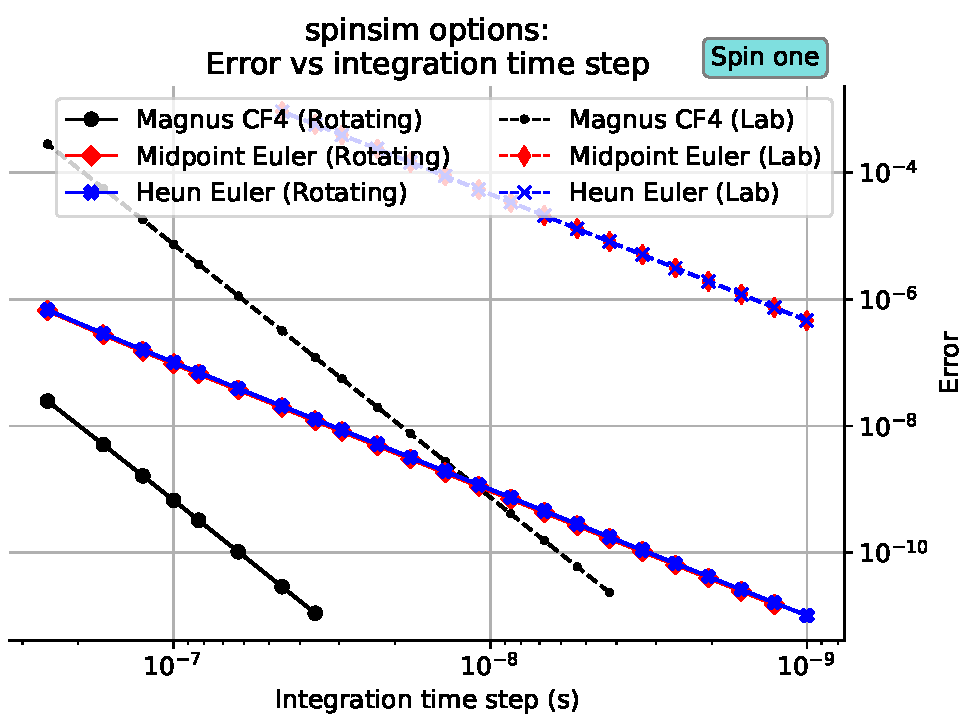
\includegraphics[scale=0.475]{benchmark_spin_one_step_error.pdf}
				% \caption{Accuracy of the spin one options of \texttt{spinsim}.}
				\caption{}
				\label{fig:benchmark_spin_one_step_error}
			\end{subfigure}
			\hfill
			\begin{subfigure}[b]{0.475\textwidth}
				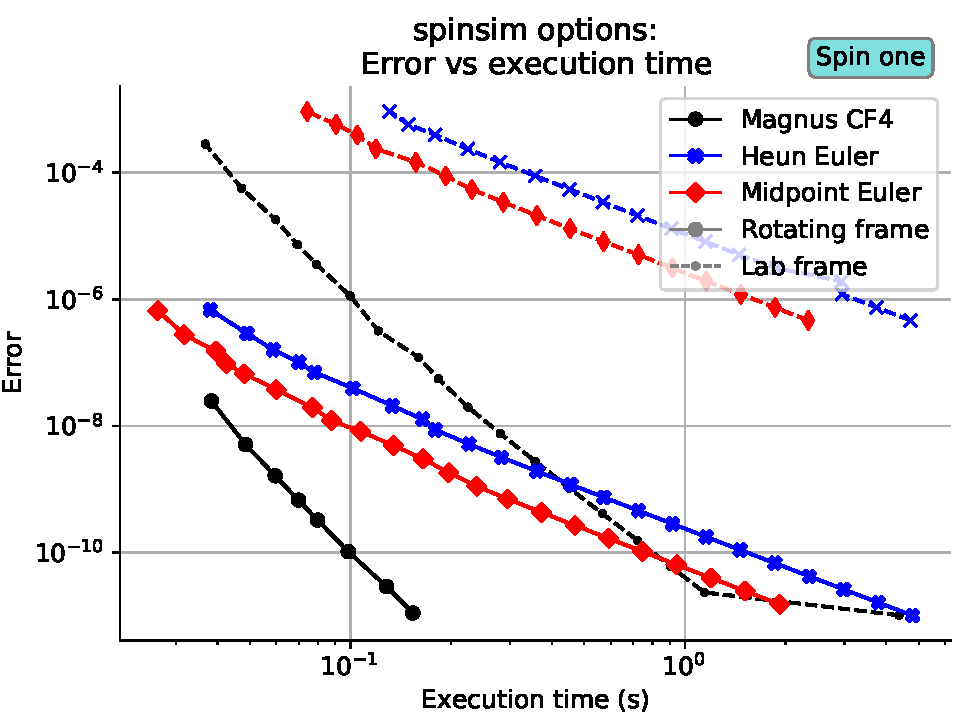
\includegraphics[scale=0.475]{benchmark_spin_one_execution_error.pdf}
				% \caption{Speed vs accuracy of the spin one options of \texttt{spinsim}.}
				\caption{}
				\label{fig:benchmark_spin_one_execution_error}
			\end{subfigure}\
			\caption{Speed and accuracy of the spin one options of \texttt{spinsim}. A simulation of a typical neural sensing experiment was run for every integration time step, for each of the possible integration techniques (Magnus based commutator free 4, and two Euler methods). In the simulation, transitions are continuously driven in the spin system for a duration of 100ms, and an additional small signal is injected for 1ms. Each technique was tested while both using and not using a transformation into a rotating frame. Both execution time and error were recorded for each of the simulations. Error is RMS error compared to a long running \emph{SciPy} baseline.}
			\label{fig:benchmark_spin_one}
		\end{figure}

		\begin{figure}[h!]
			\begin{subfigure}[b]{0.475\textwidth}
				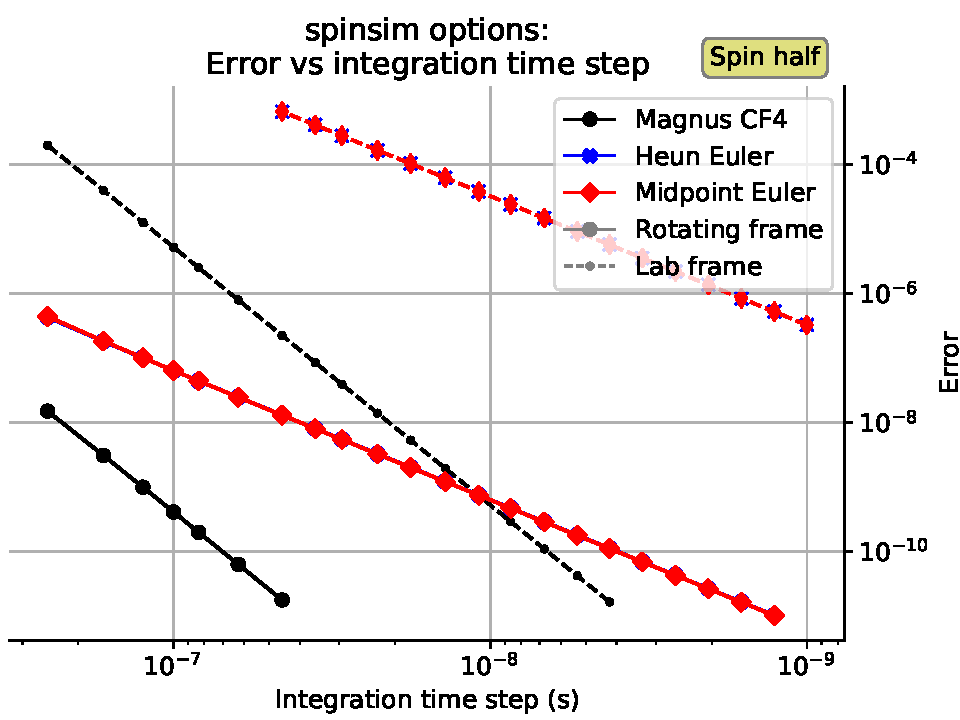
\includegraphics[scale=0.475]{benchmark_spin_half_step_error.pdf}
				% \caption{Accuracy of the spin half options of \texttt{spinsim}.}
				\caption{}
				\label{fig:benchmark_spin_half_step_error}
			\end{subfigure}
			\hfill
			\begin{subfigure}[b]{0.475\textwidth}
				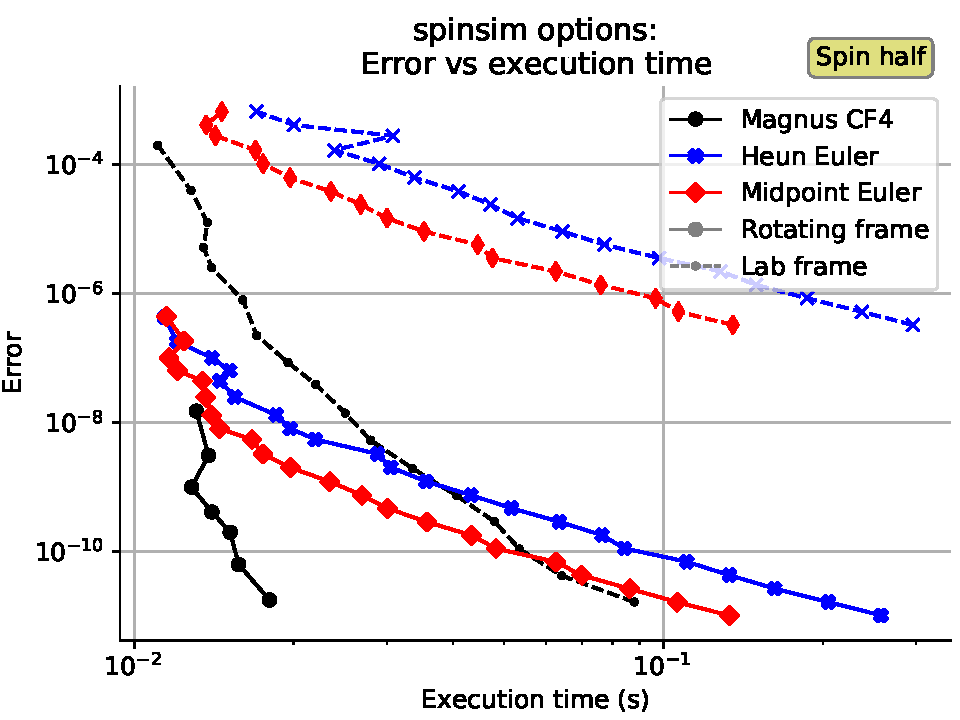
\includegraphics[scale=0.475]{benchmark_spin_half_execution_error.pdf}
				% \caption{Speed vs accuracy of the spin half options of \texttt{spinsim}.}
				\caption{}
				\label{fig:benchmark_spin_half_execution_error}
			\end{subfigure}
			\caption{Speed and accuracy of the spin half options of \texttt{spinsim}. A simulation of a typical neural sensing experiment was run for every integration time step, for each of the possible integration techniques (Magnus based commutator free 4, and two Euler methods). In the simulation, transitions are continuously driven in the spin system for a duration of 100ms, and an additional small signal is injected for 1ms. Each technique was tested while both using and not using a transformation into a rotating frame. Both execution time and error were recorded for each of the simulations. Error is RMS error compared to a long running \emph{SciPy} baseline.}
			\label{fig:benchmark_spin_half}
		\end{figure}

	\subsection{Comparison to alternatives}
		We ran the same error (using Equation \eqref{eq:error}) and execution time benchmarks on some alternative packages to compare \texttt{spinsim}'s performance to theirs. The packages compared were:
		\begin{itemize}
			\item \texttt{spinsim} running on the \emph{Cuda} device, using the CF4 integrator and the rotating frame mode, which were the highest performing options when comparing \texttt{spinsim} integration methods.
			\item \texttt{NDSolve} from the \emph{Mathematica} \cite{wolfram_research_inc_mathematica_2020} software. This was chosen as it is popular with our lab group for simulating magnetometry experiments.
			\item \texttt{scipy.integrate.ivp\_solve()} from the \emph{python} library \texttt{SciPy} \cite{virtanen_scipy_2020}. This was chosen as a generic solver from within the python ecosystem.
			\item We had also planned to benchmark against \texttt{qutip.sesolve()}, a solver in the popular quantum mechanics \emph{python} library, \texttt{QuTip} \cite{johansson_qutip_2013}. However, due to a known bug with the library’s dependencies, this was not installable on Windows 10, the operating system being used for testing, and so benchmarks for it could not be run.
		\end{itemize}

		In each case, the step sizes of the alternative integrators were limited to a maximum value obtain simulation results of different accuracies. Apart from that, the integrator settings were left untouched from the default values, as a representation of what a user would experience using a generic solver for spin system problems. Similarly to with the internal \texttt{spinsim} benchmarks, the expected spin projection was evaluated in each case, but the states were compared to calculate a relative error. Also like with the internal benchmarks, we used the longest running \emph{SciPy} simulation as a ground truth for comparison, as the accuracy of \emph{Mathematica} plateaus at small time steps.

		Each benchmark was run one simulation at a time. However, it might be possible to increase the average speed of many benchmarks from alternative packages using multithreading to run multiple benchmarks at a time. When this was attempted using \emph{Mathematica}, the kernels crashed as the 32GiB of RAM was not enough to run them all at once. Multithreading was also not attempted using \emph{SciPy}, due to the fact that running the full set of benchmarks of only a single simulation per integration time step consumes a day of computational time. But to be fair, both \emph{Mathematica} and \emph{SciPy} results are plotted with an artificial reduction in execution time by a factor of 4 and 8, which is an upper bound for the speed increase that could be obtained by running them parallel on a 4 and 8 core processor, respectively. These are respectively shown in plots as both faded and dotted lines.

		From Figure \ref{fig:benchmark_external}, for any given error tolerance, \texttt{spinsim} is over 3 orders of magnitude faster than \emph{Mathematica}, and 4 orders of magnitude more accurate than \emph{SciPy}. In practice, this means that an 8 minute \emph{SciPy} simulation is reduced to 50ms, and a full week long \emph{SciPy} batch simulation of 1000 separate systems (a realistic situation for testing quantum sensing protocols) would take less than one minute in \texttt{spinsim}.

		\begin{figure}[h!]
			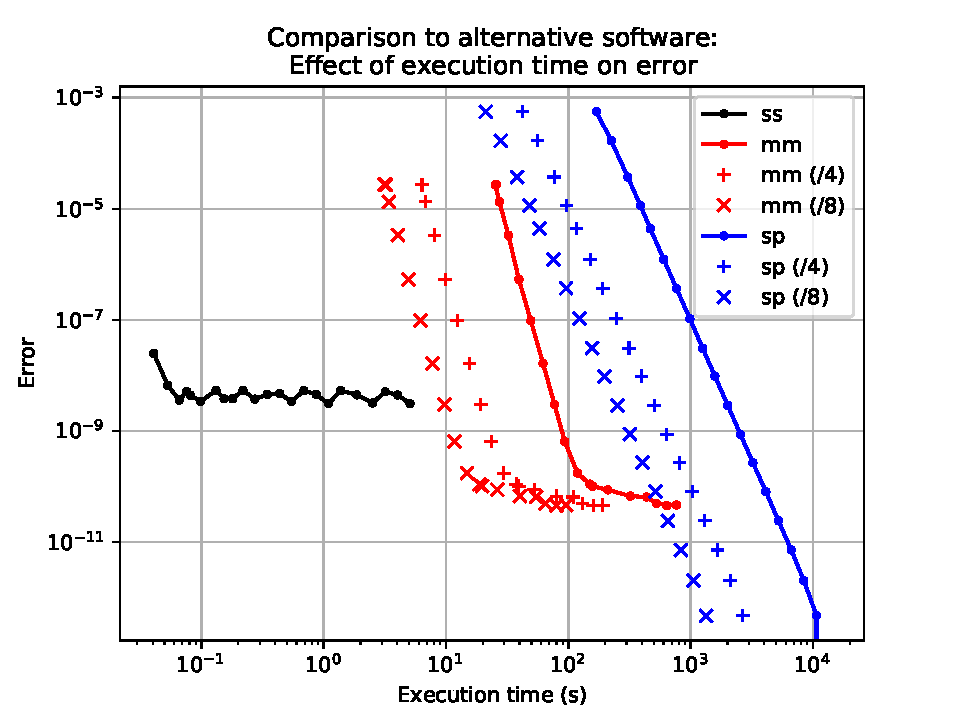
\includegraphics[scale=0.9]{benchmark_external_execution_error.pdf}
			\caption{Speed vs accuracy of two alternative integration packages. A simulation of a typical neural sensing experiment was run for every integration time step, for each of alternative packages (\texttt{NDSolve} from \emph{Mathematica}, and \texttt{scipy.integrate.ivp\_solve()} from \emph{SciPy}). In the simulation, transitions are continuously driven in the spin system for a duration of 100ms, and an additional small signal is injected for 1ms. Both execution time and error were recorded for each of the simulations. Error is RMS error compared to a long running \emph{SciPy} baseline. The \emph{Mathematica} and \emph{SciPy} results are also shown with a speed up by a factor of 4 and 8 to represent the upper bound of hypothetical parallelisation across a 4 and 8 core CPU respectively.}
			\label{fig:benchmark_external}
		\end{figure}

	\subsection{Parallelisation performance}
		Once the algorithm behind \texttt{spinsim} was developed, we wanted to check its execution speed while running on various devices. Part of this test was also to quantify the speed increase of parallelisation by comparing execution speeds on highly parallel devices (being GPUs), compared highly procedural devices (being CPUs). Speed benchmarks were performed using \texttt{sense.sim.benchmark}, by comparing evaluation speed of typical spin one sensing experiments on different devices. This is shown in Figure \ref{fig:benchmark_device_aggregate}. The integration code was compiled by \texttt{numba} for multicore CPUs, CPUs running single threaded, and \emph{Nvidia Cuda} compatible GPUs, and run on different models of each of them. These test devices are given in Table \ref{tab:devices}.

		\begin{table}[h!]
			\caption{Devices used in the parallelisation speed test. These devices are part of individual computers, which are separated here by horizontal lines.}
			\label{tab:devices}
			\begin{tabular}{l|l|l|l|l}
				\textbf{Device}	&\textbf{Type}	&\textbf{RAM (GiB)}	&\textbf{Cores}	&\textbf{Cooling}\\
				\hline
				Core i7-6700	&Intel CPU		&16					&4				&Air\\
				Quadro K620		&Nvidia GPU		&2					&384			&Air\\
				\hline
				Core i7-8750H	&Intel CPU		&16					&6				&Air\\
				GeForce GTX 1070&Nvidia GPU		&8					&2048			&Air\\
				\hline
				Ryzen 9 5900X	&AMD CPU		&32					&12				&Air\\
				GeForce RTX 3070&Nvidia GPU		&8					&5888			&Air\\
				\hline
				Ryzen 7 5800X	&AMD CPU		&32					&8				&Liquid\\
				GeForce RTX 3080&Nvidia GPU		&10					&8704			&Air\\
			\end{tabular}
		\end{table}

		\begin{figure}[htbp!]
			\centering
			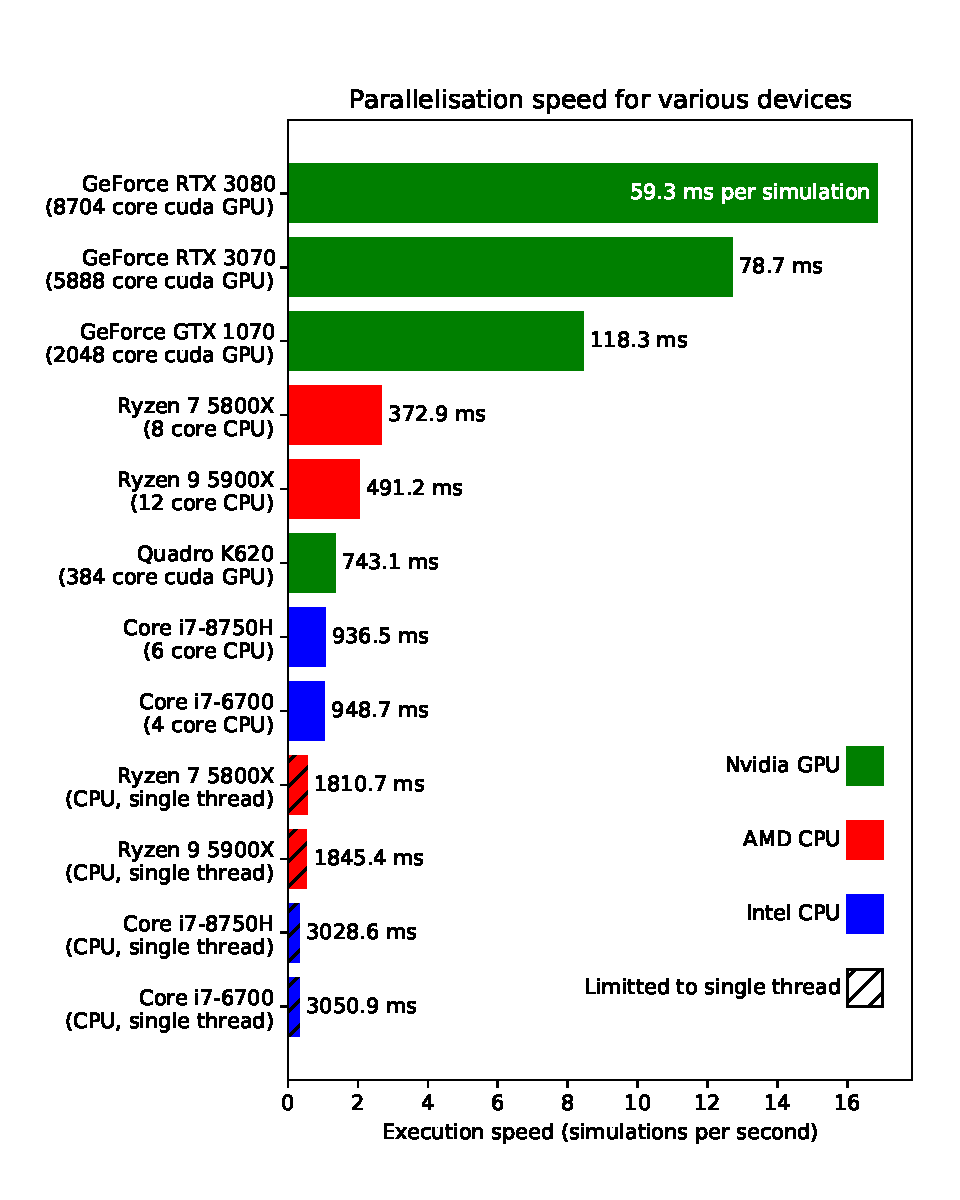
\includegraphics[scale=0.7]{benchmark_device_aggregate.pdf}
			\caption{Evaluation speed of a simulation of a typical spin one sensing experiment on both CPUs and GPUs. Integration time step is set to 100ns. Transitions are continuously driven in the spin system for a duration of 100ms, and an additional small signal is injected for 1ms. Evaluation time is determined by an average of 100 similar simulations for each device, where each individual simulation varies in dressing amplitude (transition frequency).}
			\label{fig:benchmark_device_aggregate}
		\end{figure}

		The results shown in Figure \ref{fig:benchmark_device_aggregate} show the benefit to using parallelisation when solving a spin system problem. Moving from the 6 core \emph{Core i7-8750H} CPU to the 12 core \emph{Ryzen 9 5900X} CPU doubles the execution speed, as expected. Moving from a single core processor to a high end GPU increases performance by well over an order of magnitude on three of the four computers tested on. Even the low end \emph{Quadro K620} was an improvement over the \emph{Core i7-6700} used by the same computer. Execution speed vs number of cuda cores starts to plateau as the number of cores increases. This happens as the time it takes to transfer memory from RAM to VRAM (dedicated graphics memory), which is independent on the number of cores of the GPU, becomes a comparable to the execution time of the simulator logic. However, there is still a large improvement from using the high end \emph{GeForce RTX 3070} to the \emph{GeForce RTX 3080}, with the latter simulating the experiment in almost half the time of the simulated experiment duration.

		Surprisingly, we found that the \emph{Ryzen 7 5800X} 8 core CPU was able to execute the benchmark faster than the \emph{Ryzen 9 5900X} 12 core CPU. This can be explained by the fact that the \emph{Ryzen 7 5800X} was liquid cooled, rather than being air cooled, meaning it was likely able to boost to a higher core clock, and resist thermal throttling.

		Figure \ref{fig:benchmark_device_aggregate} can be used by potential \texttt{spinsim} users for finding the relative performance for devices of varying abilities of parallelisation. We would recommend Another factor not shown in the plot is the fact that, in practice, running highly code parallel code on a CPU on a personal computer will severely limit the responsiveness of other applications, as it can utilise the entire CPU (as it should). In contrast, this does not happen when running a GPU based program, as it requires very little CPU utilisation to function. This can be convenient when running simulations on a personal laptop or desktop, as other work on the computer does not have to halt while simulations are being run.

	\subsection{Testing}
		During the accuracy tests, it was confirmed that all possible modes of \texttt{spinsim} agree with a standard \emph{SciPy} simulation up to an arbitrarily small error. The Lie Trotter matrix exponentiator was tested separately from the full system, as well as benchmarked separately. These tests and benchmarks were run as part of the \texttt{neural\_sense} package. The simulator has also been used as part of the measurement protocol being developed there, and it has been tested as part of those algorithms as well.

		The kernel execution was profiled thoroughly, and changes were made to optimise VRAM and register usage and transfer. This was done specifically for the development hardware of the \emph{GeForce GTX 1070}, so one may get some performance increases by changing some GPU specific meta parameters when instantiating the \texttt{spinsim.Simulator} object.

		A good way to confirm that \texttt{spinsim} is functioning properly after an installation is to run the tutorial code provided and compare the outputs. Otherwise, one can reproduce the benchmarks shown here using \texttt{neural\_sense.sim.benchmark}.

\section{(2) Availability}
\vspace{0.5cm}
\section{Operating system}
Developed and tested on Windows 10. CPU functionality tested on MacOS Big Sur (note that modern Mac computers are not compatible with \emph{Cuda} software). All packages referenced in \texttt{spinsim} are compatible with Linux, but functionality has not been tested.

\section{Programming language}
Python (3.7 or greater)

\section{Additional system requirements}
To use the (default) \emph{Nvidia Cuda} GPU parallelisation, one needs to have a \emph{Cuda} compatible \emph{Nvidia} GPU \cite{noauthor_cuda_2012}. For \emph{Cuda} mode to function, one also needs to install the \emph{Nvidia Cuda} toolkit \cite{noauthor_cuda_2013}. If \emph{Cuda} is not available on the system, the simulator will automatically parallelise over multicore CPUs instead.

\section{Dependencies}
numba (0.50.1 or greater)\\
numpy (1.19.3)\\
matplotlib (for example code, 3.2)\\
neuralsense (for benchmark code)

\section{List of contributors}

1. Alex Tritt\\
	School of Physics \& Astronomy, Monash University, Victoria 3800, Australia.\\
	Primary author of the released packages.\\
2. Joshua Morris\\
	School of Physics \& Astronomy, Monash University, Victoria 3800, Australia.\\
	Present address: Faculty of Physics, University of Vienna, 1010 Vienna, Austria.\\
	Author of first version of code.\\
3. Joel Hockstetter\\
	School of Physics \& Astronomy, Monash University, Victoria 3800, Australia.\\
	Present address: School of Physics, University of Sydney, NSW 2006, Australia.\\
	Optimization and extension to spin one of first version of code.\\
4. Russell P. Anderson\\
	School of Molecular Sciences, La Trobe University, PO box 199, Bendigo, Victoria 3552, Australia.\\
	Original conception of first version of code.\\
5. James Saunderson\\
	Department of Electrical and Computer Systems Engineering, Monash University, Victoria 3800, Australia.\\
	Advice on numerical analysis.\\
6. Lincoln D. Turner\\
	School of Physics \& Astronomy, Monash University, Victoria 3800, Australia.\\
	Original conception of released version of algorithm.

\section{Software location:}

{\bf Archive}

\begin{description}[noitemsep,topsep=0pt]
	\item[Name:] Monash Bridges
	\item[Persistent identifier:] 10.26180/13285460
	\item[Licence:] Apache 2.0
	\item[Publisher:]  Alex Tritt
	\item[Version published:] 1.0.0
	\item[Date published:] \textcolor{blue}{dd/mm/yy}
\end{description}

{\bf Code repository}

\begin{description}[noitemsep,topsep=0pt]
	\item[Name:] GitHub
	\item[Persistent identifier:] https://github.com/alexander-tritt-monash/spinsim
	\item[Licence:] BSD 3 Clause
	\item[Date published:] 18/11/20
\end{description}

\section{Language}

English.

\section{(3) Reuse potential}

	\subsection{Use potential and limitations}
		\texttt{spinsim} will be useful for any research group needing quick, accurate, and / or large numbers of simulations involving spin half or spin one systems. This is immediately relevant to developing new quantum sensing protocols with spin half and spin one systems. This package is being used in the context of Bose Einstein Condensate (BEC) magnetic sensing protocol design by our lab.

		This project is to be able to measure neural signals using BECs. The electrical pulses made by neurons are currently measured using electrical probes, which is intrusive and damages the cells. We instead propose to sense the small magnetic fields that these electrical currents produce. Rubidium BECs can potentially be made sensitive enough to these tiny magnetic fields that they can be measured by them. \texttt{spinsim} was written to simulate possible measurement protocols for this, showing the behaviour of the array of spin one atoms interacting with the magnetic fields of the neurons, control signals, and noise. The package is also now being used to simulate other BEC magnetometry experiments by the lab group.

		Another example of spin based magnetic field sensing is the use of Nitrogen Vacancy Centres (NVCs). These are spin one structures found in diamond doped with Nitrogen atoms. This leaves a vacancy in a position adjacent to the Nitrogen atom, which pairs of electrons occupy to obtain the spin one properties. Similar to BECs, NVCs can be placed and addressed in 2D arrays in order to take many samples in one measurement. A paper was only recently released covering simulation experiments of magnetic neural pulse sensing using NVCs \cite{parashar_axon_2020}, which is something that \texttt{spinsim} could be useful for.

		\texttt{spinsim} is designed to simulate small dimensional quantum systems, including large arrays of non-interacting spin systems. This means that it would not be able to integrate large arrays of entangled states or interacting particles. As a result, despite being fast at simulating qubits, it is inappropriate for the package to be used for quantum computing. In addition, \texttt{spinsim} is currently designed to integrate the time evolution of pure states only. This means that it may not be adequate for use in some Nuclear Magnetic Resonance (NMR) applications where relaxation \cite{veshtort_spinevolution_2006} is important (or other kinds of simulations involving decoherence).

		With these restrictions in mind, \texttt{spinsim} could be used for some simplified simulations in various areas of NMR. There are many atomic nuclei with spins of half (eg protons, Carbon 13) and, and fewer that have spins of one (eg Lithium 6, Nitrogen 14) \cite{fuller_nuclear_1976}, which, if relaxation and interactions between systems are not important for the application, \texttt{spinsim} could be used to simulate for spectroscopy experiments, for example. The inclusion of a quadrupole operator means that, with the same level of simplifications, \texttt{spinsim} should be able to simulate Nuclear Quadrupole Resonance (NQR) spectroscopy for spin one nuclei \cite{bain_nqr_2004}, such as Nitrogen 14, provided a suitable coordinate system is chosen. This technique measures energy level differences between levels split by electric field gradients, rather than static magnetic bias fields. Another possible use case could be for Magnetic Resonance Imaging (MRI) simulation and pulse sequence design. MRI uses measures the response of spins of an array of spin half protons to a spatially varying pulse sequence \cite{mckinnon_physics_1998}, which essentially just corresponds to many separate \texttt{spinsim} simulations of spins at different positions in space. While this package offers some advantages over state of the art simulators in the field \cite{kose_fast_2019}, with its use of quantum mechanics over classical mechanics, and its absence of rotating wave approximations, its parametrised pulse sequence definitions and geometric integrator, again, the lack of interacting particles and decoherence features are may limit its use in this area.

	\subsection{Support}
		Documentation for \texttt{spinsim} is available on \href{https://spinsim.readthedocs.io/en/latest/}{\emph{Read the Docs}}. This documentation contains a thorough tutorial on how to use the package, and installation instructions.
		
		For direct support with the \texttt{spinsim} package, one can open an issue in the \emph{github} repository. One can also use this contact to suggest extensions to the package. \texttt{spinsim} is planned to be maintained by the Monash University spinor BEC lab into the future.

\section{Acknowledgements}

Thank you to the Monash University School of Physics and Astronomy spinor BEC lab group, particularly Hamish Taylor and Travis Hartley, who have started using \texttt{spinsim} for their own projects and have given useful feedback of their user experience with the package.

\section{Funding statement}

\textcolor{blue}{If the software resulted from funded research please give the funder and grant number.}

\section{Competing interests}

The authors declare that they have no competing interests.

\bibliography{spinsim}{}
\bibliographystyle{vancouver}

\vspace{2cm}

\rule{\textwidth}{1pt}

{ \bf Copyright Notice} \\
Authors who publish with this journal agree to the following terms: \\

Authors retain copyright and grant the journal right of first publication with the work simultaneously licensed under a  \href{http://creativecommons.org/licenses/by/3.0/}{Creative Commons Attribution License} that allows others to share the work with an acknowledgement of the work's authorship and initial publication in this journal. \\

Authors are able to enter into separate, additional contractual arrangements for the non-exclusive distribution of the journal's published version of the work (e.g., post it to an institutional repository or publish it in a book), with an acknowledgement of its initial publication in this journal. \\

By submitting this paper you agree to the terms of this Copyright Notice, which will apply to this submission if and when it is published by this journal.


\end{document}
